\documentclass{beamer}
\usepackage[utf8]{inputenc}
\usepackage{url}
\usepackage{hyperref}
\graphicspath{{./fig/aula5}}

% Configurando layout para mostrar codigos C++
\usepackage{listings}
\lstset{
  language=HTML,
  basicstyle=\ttfamily\small, 
  keywordstyle=\color{blue}, 
  stringstyle=\color{red}, 
  commentstyle=\color{red}, 
  extendedchars=true, 
  showspaces=false, 
  showstringspaces=false, 
  numbers=left,
  numberstyle=\tiny,
  breaklines=true, 
  backgroundcolor=\color{green!10},
  breakautoindent=true, 
  captionpos=b,
  xleftmargin=0pt,
}


\title{Desenvolvimento Web Básico}
\subtitle{Aula 5}

\usetheme{lucid}

\begin{document}
\frame{
 \titlepage
}

%--------------------------------------------------------------------------
\begin{frame}{Na aula de hoje...} 
\tableofcontents 
\end{frame}
%--------------------------------------------------------------
\section{Arrays}
\begin{frame}{Vetores JS}
Declarando um array JS.
\begin{itemize}
    \item Crie um arquivo aula5.js;
    \item Executaremos o arquivo via comando \textbf{node aula5.js}
    \item Usa-se \textbf{const};
    \item É instanciado um objeto da classe Array;
\end{itemize}
  \begin{center}
       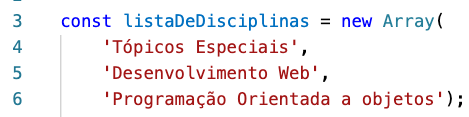
\includegraphics[height=0.2\paperheight]{fig/aula5/aula_js_5_1.png} \\
       \tiny{\textbf{Fonte: } A autora.}
      \end{center}
\end{frame}
%---------------------------------------------------------------------------------
\begin{frame}{Manipular Array JS}
Imprimir um vetor em Java Script é simples;
\lstinputlisting[linerange={13-13}]{cod/aula5_listas.js}
Acrescentando um elemento no vetor; 
\lstinputlisting[linerange={10-10}]{cod/aula5_listas.js}
\end{frame}
%---------------------------------------------------------------------------------
\begin{frame}{Manipular Array JS}
Remover o elemento de um vetor, usa-se \textbf{splice};
\lstinputlisting[linerange={12-12}]{cod/aula5_listas.js}\\
Os valores indicam o índice onde inicia a seleção e a quantidade de elementos removidos.\\
\paragraph{Exibir um elemento do vetor usa-se vetor[índice]}
\lstinputlisting[linerange={14-14}]{cod/aula5_listas.js}
\cite{wschool2018js}
\end{frame}
%-----------------------------------------------------------------
\section{Atividade de aula}
\begin{frame}{Atividade}
  \begin{enumerate}
      \item Seguindo os passos da aula, livros indicados e, a leitura adicional recomendada: 
      \item Uma página que receba valores via input e adicione cada valor a uma posição de um array;
      \item Exiba o array em um outro elemento da página;
  \end{enumerate}


\end{frame}
%----------------------------------------------------------------------------
\section{Referências}

\begin{frame}{Referências}%[allowframebreaks]
\small
\begin{center}
\tiny
\bibliographystyle{apalike}
\bibliography{ref_aula}
\end{center}
\end{frame}

\end{document}

\end{document}